\PassOptionsToPackage{pdfpagelabels=false}{hyperref} 
\documentclass{sigchi}

% Use this command to override the default ACM copyright statement
% (e.g. for preprints).  Consult the conference website for the
% camera-ready copyright statement.

%% EXAMPLE BEGIN -- HOW TO OVERRIDE THE DEFAULT COPYRIGHT STRIP -- (July 22, 2013 - Paul Baumann)
% \toappear{Permission to make digital or hard copies of all or part of this work for personal or classroom use is      granted without fee provided that copies are not made or distributed for profit or commercial advantage and that copies bear this notice and the full citation on the first page. Copyrights for components of this work owned by others than ACM must be honored. Abstracting with credit is permitted. To copy otherwise, or republish, to post on servers or to redistribute to lists, requires prior specific permission and/or a fee. Request permissions from permissions@acm.org. \\
% {\emph{CHI'14}}, April 26--May 1, 2014, Toronto, Canada. \\
% Copyright \copyright~2014 ACM ISBN/14/04...\$15.00. \\
% DOI string from ACM form confirmation}
%% EXAMPLE END -- HOW TO OVERRIDE THE DEFAULT COPYRIGHT STRIP -- (July 22, 2013 - Paul Baumann)

% Arabic page numbers for submission.  Remove this line to eliminate
% page numbers for the camera ready copy
% \pagenumbering{arabic}

% Load basic packages
\usepackage{balance}  % to better equalize the last page
\usepackage{graphics} % for EPS, load graphicx instead 
\usepackage[T1]{fontenc}
\usepackage{txfonts}
\usepackage{mathptmx}
\usepackage{pgfplots}
\usepackage{pgf-pie}
\usepackage{tikz}
\usepackage{environ}
\usepackage{tikzscale}
\usepackage{comment}
\usepackage{amssymb}
\usepackage{wrapfig}
\usepackage{booktabs}
\usepackage{framed}


\usepackage{subcaption}

\usepackage{verbatim}


\pgfplotsset{compat=1.8}
\usepgfplotslibrary{statistics}


\usepackage[pdftex]{hyperref}
\usepackage{color}
\usepackage{booktabs}
\usepackage{textcomp}
% Some optional stuff you might like/need.
\usepackage{microtype} % Improved Tracking and Kerning
% \usepackage[all]{hypcap}  % Fixes bug in hyperref caption linking
\usepackage{ccicons}  % Cite your images correctly!
% \usepackage[utf8]{inputenc} % for a UTF8 editor only

% If you want to use todo notes, marginpars etc. during creation of your draft document, you
% have to enable the "chi_draft" option for the document class. To do this, change the very first
% line to: "\documentclass[chi_draft]{sigchi}". You can then place todo notes by using the "\todo{...}"
% command. Make sure to disable the draft option again before submitting your final document.
\usepackage{todonotes}

% Paper metadata (use plain text, for PDF inclusion and later
% re-using, if desired).  Use \emtpyauthor when submitting for review
% so you remain anonymous.
\def\plaintitle{Slide: Fast Text Input in Virtual Reality}
\def\plainauthor{First Author, Second Author, Third Author,
  Fourth Author, Fifth Author, Sixth Author}
\def\emptyauthor{}
\def\plainkeywords{virtual reality; text input; text entry; multimodal.}
\def\plaingeneralterms{Documentation, Standardization}

% llt: Define a global style for URLs, rather that the default one
\makeatletter
\def\url@leostyle{%
  \@ifundefined{selectfont}{
    \def\UrlFont{\sf}
  }{
    \def\UrlFont{\small\bf\ttfamily}
  }}
\makeatother
\urlstyle{leo}

% To make various LaTeX processors do the right thing with page size.
\def\pprw{8.5in}
\def\pprh{11in}
\special{papersize=\pprw,\pprh}
\setlength{\paperwidth}{\pprw}
\setlength{\paperheight}{\pprh}
\setlength{\pdfpagewidth}{\pprw}
\setlength{\pdfpageheight}{\pprh}

% Make sure hyperref comes last of your loaded packages, to give it a
% fighting chance of not being over-written, since its job is to
% redefine many LaTeX commands.
\definecolor{linkColor}{RGB}{6,125,233}
\hypersetup{%
  pdftitle={\plaintitle},
% Use \plainauthor for final version.
%  pdfauthor={\plainauthor},
  pdfauthor={\emptyauthor},
  pdfkeywords={\plainkeywords},
  bookmarksnumbered,
  pdfstartview={FitH},
  colorlinks,
  citecolor=black,
  filecolor=black,
  linkcolor=black,
  urlcolor=linkColor,
  breaklinks=true,
}

% create a shortcut to typeset table headings
% \newcommand\tabhead[1]{\small\textbf{#1}}

% End of preamble. Here it comes the document.
\begin{document}

\title{\plaintitle}
\def\emptyauthor{}
\begin{comment}
\numberofauthors{3}
\author{%
  \alignauthor{Leave Authors Anonymous\\
    \affaddr{for Submission}\\
    \affaddr{City, Country}\\
    \email{e-mail address}}\\
  \alignauthor{Leave Authors Anonymous\\
    \affaddr{for Submission}\\
    \affaddr{City, Country}\\
    \email{e-mail address}}\\
  \alignauthor{Leave Authors Anonymous\\
    \affaddr{for Submission}\\
    \affaddr{City, Country}\\
    \email{e-mail address}}\\
}
\end{comment}
\maketitle

\begin{abstract}

Text input in VR is challenging because of the latency in visual feedback and the lack of proprioception.  Our design Slide, a virtual keyboard that requires only a track pad, is based on 3 concepts: (1) relative vectors: to enter a character, the user slides from what is assumed to be the center of the keyboard to the key of interest.  (2) directional, with error correction: all keys are grouped in 6 tiles, and the user only has to slide in the direction of the tile containing the key.  A Bayesian word recommender determines the word entered. (3) Intention-based hybrid keyboard: the keyboard automatically switches between the 26-key and 6-tile keyboard based on the user's finger movements.   Our user study suggests that Slide can be learned quickly, and delivers an average text entry speed of 34 words per minute with an error rate of 4\%.  

\begin{comment}
 is able to be learned quickly by beginners and supports eyes-free entry by experts.  The participants are able to type an average text entry speed of Y WPM with an error rate of Z\%.  These results show that text entry is similar to that of a mobile phone keyboard but error correction and editing, the most time consuming step, is greatly improved.
\end{comment}
\end{abstract}

\category{H.5.1.}
{Information Interfaces and Presentation (e.g. HCI)}
{Multimedia Information Systems}
\category{I.3.7.}
{Computer Graphics}
{Three-Dimensional Graphics and Realism}

%link at: http://www.acm.org/about/class/ccs98-html

\keywords{\plainkeywords}



\section{Introduction}
%architectural reviews,~\cite{guerreiro2014beyond}, large group chats ~\cite{mcnerney1999system}, data visualization~\cite{abbott2011empire}

While the primary use of virtual reality is in games and videos today, it can be used in numerous application domains, from education, architectural reviews, healthcare, large group chats, and data visualization, exploration of space and other dangerous locations, scientific visualization, manufacturing, journalism, traveling, architecture, and shopping.  

Virtual reality (VR) systems have become available to the general public recently and the virtual reality controllers introduced by HTC, Facebook, and Google have similar characteristics. 
Each includes a controller, shown in Figure~~\ref{fig:controllers}.
The Daydream controller, shown in Figure~\ref{fig:controllerDaydream}, in only for a single hand whereas the others have a controller for each hand.  The three major controllers all contain a way to track the thumb, at least 3 degrees of freedom tracking  (rotational), and at least four buttons.
Vive (\subref{fig:controllerVive}) and Oculus (\subref{fig:controllerOculus}) use an absolute tracking system to minimizing sensor drift and to allow for rotational and translational tracking~\cite{hilfert2016low}.  The Vive and Daydream (\subref{fig:controllerDaydream}) employ a thumb track pa!d to capture finger movement.  Oculus controller uses joysticks instead. 

\begin{figure}
  \centering
	\begin{subfigure}{.4\columnwidth}
  \includegraphics[width=\textwidth]{figures/controllerVive}
  \caption{HTC's Vive }\label{fig:controllerVive}
  \end{subfigure}
  \\
  \begin{subfigure}{.4\columnwidth}
  \includegraphics[width=\textwidth]{figures/controllerOculus}
  \caption{Facebook's Oculus}\label{fig:controllerOculus}
  \end{subfigure}
  \\
  \begin{subfigure}{.4\columnwidth}
  \includegraphics[width=\textwidth]{figures/controllerDaydream}
  \caption{Google's Daydream}\label{fig:controllerDaydream}
  \end{subfigure}
  \caption{Virtual reality controllers}
~\label{fig:controllers}

\end{figure}

Even though typing is not prevalent in immersive virtual reality, text entry is still important, with a wide range of uses: from typing in account names and passwords, searching items, specifying parameters used in the applications, referring to friends,  writing notes and chatting with others, etc.      

The average typing performance on a regular keyboard was found to be about 60 words per minute\cite{varcholik:textentry}, thanks to the dexterity of our fingers, the haptic feedback from the physical keyboards, and visual feedback on the display.    In the context of virtual reality, it is often not an option to use a physical keyboard.  We are usually not sitting down and it is hard to switch between the VR controllers and a physical keyboard, further complicated by the fact that we cannot see the keyboard in VR.  To avoid having to remove the head gear to type, it is desirable to enter text using existing VR controllers. 

Typing is challenging in virtual reality because of the latency in visual feedback and the lack of proprioception.  The industry standard is to enter text with gaze.  A virtual keyboard is presented in VR, and users type a letter by gazing at the desired key and tapping on the controller.   It was found that the users can typically type at about 7 words per minute~\cite{majaranta2006effects}.   Entering text via speech is attractive, especially in the immersive virtual reality environment.  Speech may not be suitable when entering names and URLs, especially in public spaces due to privacy issues.  Furthermore, speech often needs to be corrected via text editing.  Other alternatives proposed including using gesture, motion controllers, Leap Motion or tangibles, handheld controllers, or relying on a subset of keyboard and mouse commands~\cite{billinghurst1999collaborative}.
All these existing solutions, while potentially good for simple tasks, aren't adequate for tasks that requires a greater bandwidth of input~\cite{McGill:2015:DRO:2702123.2702382}.


\subsection{Methodology}

The goal of the paper is to understand how we can enter text simply, quickly, and accurately via the touchpad found in commodity VR controllers today.  
\begin{enumerate}
\item
We started our investigation by exploring existing ideas:
\begin{enumerate}
\item
Gazing.  Users enter keys by gazing at the keys in a virtual keyboard. 

\item
Drumming.  Keys are displayed as a virtual drum kit, users enter keys by hitting the corresponding drums using the controllers as drumsticks\cite{Google:VRdrum}. 

\item
Augmented reality.  A camera is used to stream the view of the touchpad and fingers into
virtual reality.  

\item
26-key tapping.  Users use the touchpad to tap on the virtual keyboard displayed in the VR. 

\item
26-key swiping.  Users use the touchpad to swipe on the virtual keyboard displayed in the VR. 
\end{enumerate}
We built a prototype of each of these systems and tested it informally on 3 to 5 users.  This study revealed major deficiencies in each of these approaches.  

\item
We propose a new virtual keyboard, Slide, that incorporates the learning from our initial investigation.  It is based on three main design concepts: 
\begin{enumerate}
\item
Relative vectors.  To enter a character, the user slides from what is assumed to be the center of the keyboard to the key of interest.  

\item
Directional input, with error correction.  All keys are grouped in 6 tiles, and the user only has to slide in the direction of the tile containing the key.  A Bayesian word recommender determines the word entered. 

\item
Intention-based hybrid keyboard: the keyboard automatically switches between the 26-key and 6-tile keyboard based on the user's finger movements.  
\end{enumerate}

\item 
We implemented the proposed technique in the Vive system; note that Slide is applicable to the other VR controllers as well.   We conducted a study with 15 users and evaluated the speed, accuracy, as well as the learnability of the system. 
\end{enumerate}

\subsection{Contribution}
This paper proposes Slide, a VR text entry technique that requires only a touch pad.  To address the visual latency and lack of proprioception in VR, we have adopted relative positioning with a heavy use of auto-correction.  The virtual keyboard is divided into six tiles placed around the center of the keyboard.  The user needs to slide his finger in one of the six directions towards the tile containing the character, and error correction is used to pick the most likely word.  Our study shows that users can type at the speed of 34 words per minute on average, with an error rate of 4\%.   

Slide allows for graceful degradation, when better control over the text entry is necessary, such as for typing in passwords.  The user can fall back to sliding to the precise key; our keyboard automatically detects the use of the more precise mode by observing the speed of the sliding motion.  The users can type at about 12 words per minute using this slow but more precise entry method.


\section{Related Work}

In this section, we discuss studies applicable to virtual reality based text entry.
For a full review of text entry methods, see~\cite{mackenzie2002text, zhai2005search, Buxton2011}.

\subsection{Novel QWERTY Keyboards}
Researchers have leveraged a users' familiarity with the QUERTY~\cite{noyes1983qwerty} keyboard to make their novel devices easier to use.
The Half-QWERTY keyboard~\cite{matias1993half} is arm-mounted and has a reduced size by using only half of a QWERTY keyboard.
The Pinch Gloves~\cite{bowman2002text} controls a virtual keyboard with hand rotations and finger-mounted buttons.
Another glove, KITTY~\cite{Kuester:2005:TKI:1101616.1101635} uses the tapping of contacts on each finger with the thumb to mimic a keyboard.
DigiTap~\cite{Pratorius:2014:DEV:2671015.2671029} is a similar idea but uses a wrist mounted camera instead of a glove.

\subsection{Word Gesture Keyboards}
Word gesture keyboards such as ShapeWriter~\cite{zhai2012word,Zhai:2009:SIL:1520340.1520380} and SHARK 2~\cite{kristensson2004shark}, are gesture based text input methods.
Words are written through a gesture that links the letters of the intended word on a soft keyboard. A language model and word prediction is required to select the most likely word from  candidate words.
For out of vocabulary and hard-to-predict words, a deterministic input method is still needed.
VelociTap~\cite{vertanen2015velocitap} takes the predictive model further by only predicting the whole sentence.

\subsection{Gloves and Chording Keyboards}
Other approaches abandon the QWERTY keyboard entirety.
Chording keyboards~\cite{noyes1983chord}, such as Twiddler~\cite{lyons2004twiddler} use a combination of a few keys to produce characters.
Chording is done is done with gloves, such as Chording Glove~\cite{rosenberg1999chording}.
The VirtualPhonepad~\cite{ahn2006virtualphonepad} imitates text entry via a $3\times3$ mobile phone keypad.
Virtual Notepad~\cite{poupyrev1998virtual} allows for creating handwritten annotations in virtual reality.
Connecting the Dots~\cite{frees2006connecting} approximates handwriting by having users connect dots on a $3\times3$ virtual dot matrix to scribe a single character.

In a literature review, the Pinch Gloves, pen and tablet, chording keyboard, and a speech-based are compared~\cite{bowman2002text}.
The pen and tablet and speech are fastest.  The pen and tablet had the fewest errors.
The comparison was done before specialized virtual reality input device were invented.

\subsection{Home Entertainment Input Devices}
Text entry methods is sought after in other application areas, such as home entertainment systems.
SpeeG~\cite{hoste2012speeg} is a Kinect~\cite{geerse2015kinematic} version of Speech Dasher~\cite{vertanen2010speech} text input technique.
The user speaks and then corrects mistakes using an interface that scrolls through the recognized text as well as alternatives.
SpeeG2~\cite{hoste2013speeg2} uses a grid instead of a scroll.

\subsection{Speech recognition}
Spoken language is effective for human-human interaction but often has severe limitations when applied to human-computer interaction.
Speech is slow for presenting information and interferes significantly with other cognitive tasks~\cite{shneiderman2000limits}.

Speech recognition is limited when typing passwords, names, and URLs~\cite{TODO}. 
The lack of user acceptance is also due to issues such as privacy, the perception of bothering others, the awkwardness of speaking to a machine~\cite{sawhney2000nomadic}.
Some users find voice as unreliable especially when the accent or ambient sound negatively affect accuracy.
Studies have shown that users find it ``harder to talk and think than type and think" and considered the keyboard to be more ``natural" than speech for text entry ~\cite{Karat:1999:PEC:302979.303160}.

In virtual reality, a Japanese speech-based entry system represents candidate words recognized by the speech recognition engine as blocks that can be moved around in the virtual enviroment~\cite{osawa2002multimodal}. 

For mobile phones, speech entry is three times faster than typing for English and Mandarin~\cite{ruan2016speech}.  
In this experimental setup, participants were given a set of phrases to type and speak.
The phrases are given ahead of time, but normal speech is filled with hesitations, repetitions, changes of subject in the middle of an utterance~\cite{forsberg2003speech} as the user thinks.
This could lead to an unrealistic accuracy for speech.  
The study also excludes punctuation marks and capital letters from the phrases.
Generating accurate punctuation  automatically with speech input is not yet possible and must be done manually~\cite{chen1999speech}.

\subsection{Gaze Directed Typing}
Gaze directed typing is the main text input method used today in systems such as Oculus G earVR. A main advantage of this method is that it uses the available hardware and does not require an additional device. This method is slow~\cite{card1983psychology, mackenzie1992fitts} and inconvenient since the whole head has to be moved for each character.
Moving the head while the VR scene remains static also often causes nausea or dizziness~\cite{atienza2016interaction}.   

\subsection{Text Input with Virtual Reality Controllers}
While early, input methods and controllers are being developed specifically for use in virtual reality.
FaceTouch~\cite{Gugenheimer:2016:FTI:2851581.2890242} has the backside of the head mounted display that as a touch sensitive surface.
The user selects virtual content by touching the corresponding location on backside of the display.
It is useful but only for short periods of time before the users' arms get tired.

Belt~\cite{dobbelstein2015belt} is a novel unobtrusive input device for wearable displays that has a touch surface encircling a users' hip.
The wide input space for a horizontal spatial mapping but suffers from low throughput, arm fatigue, and social acceptance.
Nenya~\cite{ashbrook2011nenya} uses a finger ring as an input mechanism that is always available.
It is fast to access, allows analog input, and is socially acceptable by being embodied in a commonly worn item.

Industry has started to standardize around a virtual reality controller.  HTC, Facebook, and Google have all released a virtual reality hardware design.
Each includes a controller, shown in Figure~~\ref{fig:controllers}.
They all similar in the they all contain a rotational tracking, a way to track the thumb through either joystick or touchpad, and at least four buttons.
Vive and Oculus use an absolute tracking system to minimizing sensor drift and to allow for rotational and translational tracking~\cite{hilfert2016low}.
The Daydream controller, shown in Figure~\ref{fig:controllerDaydream}, in only for a single hand whereas the others have a controller for each hand.
SwipeVR is implemented using the Vive but could be implemented on the other two.

\newcommand{\ra}[1]{\renewcommand{\arraystretch}{#1}}


\begin{table*}\centering
\ra{1.3}
\begin{tabular}{@{}rrrrrr@{}}\toprule
						& $Speech$ 		& $Gaze$ 		& $Mobile$		& $SwipeVR$  \\
\midrule
$Positioning$			&				& absolute		& absolute		& relative	  		\\
$Hardware$ 				&microphone 	& HMD \& button	& touch screen	& controller		\\
$Keys$ 					&				& 26+			& 26+			& 6					\\
$Special~Characters$ 	&				& \checkmark	& \checkmark	& \checkmark		\\
$Granulatiry$ 			&word			& character		& character		& word or character	\\
$Hands$ 				& 0				& 1				& 1 or 2		& 1					\\
$Real-Time~Feedback$ 	& word			& character		& character		& word				\\
$Cursor~Mode$ 			& NA			& persistent	& NA			& snap-to-home		\\
$Silent$ 				&				& \checkmark	& \checkmark	&\checkmark			\\
$Muscle$ 				& vocal chords	& neck			& fingers		& thumb			\\
$WPM$					& \%\cite{sppechTBA} & \%		& \%			& \%\\
$Error~Rate$			& \%\cite{sppechTBA} & \%		& \%			& \%\\

%    Correction Method		& X 			& X 			& X				& 	\checkmark		\\ 

\bottomrule
\end{tabular}
\caption{Ontology of input methods.}
\label{table:ontology}
\end{table*}

\begin{figure}
  \centering
	\begin{subfigure}{.4\columnwidth}
  \includegraphics[width=\textwidth]{figures/controllerVive}
  \caption{HTC's Vive }\label{fig:controllerVive}
  \end{subfigure}
  \\
  \begin{subfigure}{.4\columnwidth}
  \includegraphics[width=\textwidth]{figures/controllerOculus}
  \caption{Facebook's Oculus}\label{fig:controllerOculus}
  \end{subfigure}
  \\
  \begin{subfigure}{.4\columnwidth}
  \includegraphics[width=\textwidth]{figures/controllerDaydream}
  \caption{Google's Daydream}\label{fig:controllerDaydream}
  \end{subfigure}
  \caption{
  Industry is standardizing on some of the important components for virtual reality controllers.
  The three major controllers shown above all contain a way to track the thumb, at least 3 degrees of freedom tracking  (rotational), and at least four buttons.
  The Vive (\subref{fig:controllerVive}) and the Oculus (\subref{fig:controllerOculus}) use room-scale tracking to give 6 degrees of freedom (rotation and translation).  
  Many virtual reality systems today are released with a controller for each hand.  
  The Vive and Daydream (\subref{fig:controllerDaydream}) employ a thumb track pad to capture finger movement.
  Oculus controller uses joysticks instead.
  The system described in this paper is implemented using the Vive and could be implemented on the other two.
  }~\label{fig:controllers}

\end{figure}




\section{Exploring the Design Space of Text Input in VR}

\subsection{Challenges of Text Entry in Virtual Reality}

Text entry using a physical keyboard is a complex interaction that involves the placement of the user's hands, the kinaesthetic feedback of fingers, and the physical constraints of the keyboard~\cite{McGill:2015:DRO:2702123.2702382}.
Together this interaction is able to create an efficient text entry mechanism.

However, in the context of virtual reality, it is often not possible to use a physical keyboard.
Additionally, it is desirable to be able to type with existing virtual reality specific input devices, so the user doen't have to remove the head-mounted display to type. 
In this next section we explore the challenges of text in virtual reality.

\subsubsection{Latency in Visual Feedback}
Typing is complex interaction that requires a high-bandwidth feedback loop~\cite{McGill:2015:DRO:2702123.2702382}.
Latency is a barrier in achieving a seamless interaction between the real and virtual~\cite{leedesigning}.

In virtual reality, latency is the time between movement of the and the updated image being displayed on the screen.  
This pipeline includes the times for fusion, image transmission, rendering, sensor response and display response.
This is commonly referred to as the \textit{motion-to-photon} latency.

To achieve a genuine sense of presence~\cite{schuemie2001research} in virtual reality, the total \textit{motion-to-photon} latency must be less than 20 milliseconds~\cite{jerald2009relating,jerald2010scene,bailey2004latency}.
Some existing systems have a latency as high as 80 milliseconds ~\cite{lincoln2016motion,dallaire2016animated}.

Compared to head movement, touch-based interactions need even tighter tolerances on latency.
Research on touchscreens finds that for a user to perceive display elements as naturally being affected by touch, there is a perceptual floor between 2  and 11 milliseconds below which users do not notice lag~\cite{Jota:2013:FFE:2470654.2481317,Ng:2012:DLD:2380116.2380174}.
Further, for dragging interactions, a latency of 2.38 milliseconds is required to give the perception of a natural interaction~\cite{Jota:2013:FFE:2470654.2481317,Ng:2012:DLD:2380116.2380174}.

\subsubsection{Limited Proprioception}
Manipulation in virtual reality is difficult because users must do without the haptic contact with keyboard buttons they rely on in the real world to orient themselves.
Interactions involving the body and the external world become difficult.
For example, even the simple task of placing the finger on the correct key can become difficult given the lack of proprioceptive sensations in virtual reality.

\subsubsection{Reduced Precision}
Haptic feedback and physical constraints in real world input devices help to define interactions. 
Fine-grained control is difficult in virtual reality and restricts users to the coarse manipulation of virtual objects.
Input devices that excluded the use of the fingers are slower~\cite{Zhai:1996:IMG:238386.238534}.  

\subsection{Initial Experimentation}

Our exploration of virtual reality input methods starts by building a few prototypes.
With each prototype, we ask 3 to 5 users to type a few sentences.  
For each test we give little to no instruction about how the input method works and try to let the user interact with it naturally.
The goals of this prototyping process is to explore the performance potential of each input device and to investigate if users could understand the visual interface.
We record typing speeds, their understanding of the input device, and their verbal feedback.

\subsection{Design \#1 - Gaze Input}
Many virtual reality apps today use a gaze keyboard for text entry~\cite{netflix_app_for_oculus}.
A virtual keyboard is presented in virtual reality.
The users types a letter by gazing at the desired key and tapping on a button located on the side of the head mounted display.
Users find the process slow and the motion of the head with the fixed keyboard can causes nausea and dizziness~\cite{atienza2016interaction}.
We found users type around 10 words per minute using this method.

\subsection{Design \#2 - Drumming}
Google models typing as drumming~\cite{google_drums}.
Controllers in the real world are mapped to drum sticks in the virtual world.  
Typing a character means hitting one of 26 drums laid out like a keyboard.
Users find it fun.
It could be difficult to hit the correct key and the constant arm movement some users found to be strenuous.
We found users type around 20 words per minute using this method.

\subsection{Design \#3 - External Camera}

We next explore the use of a virtual keyboard on a touchscreen, the input method used on mobile phones today.
To address the problem that we cannot see our fingers in virtual reality, we experimented with mixed reality (augmented plus virtual) with a camera.
Our prototype points the front facing camera on the head mounted display points at the mobile keyboard, and streams the view of our fingers and the keyboard into the virtual environment. 

The goal of this prototype is to investigate how latency and presence, particular of the fingers, affect performance.
We found that the latency is an inhibitor to fast input.
Our fingers are so fast that we can only see where our fingers were.
What we see is constantly wrong and just makes it even harder to type.
This prototype demonstrates how challenging the visual latency is for typing. 
We found users type around 10 words per minute using this method.


\begin{figure}[!htb]
  \centering

  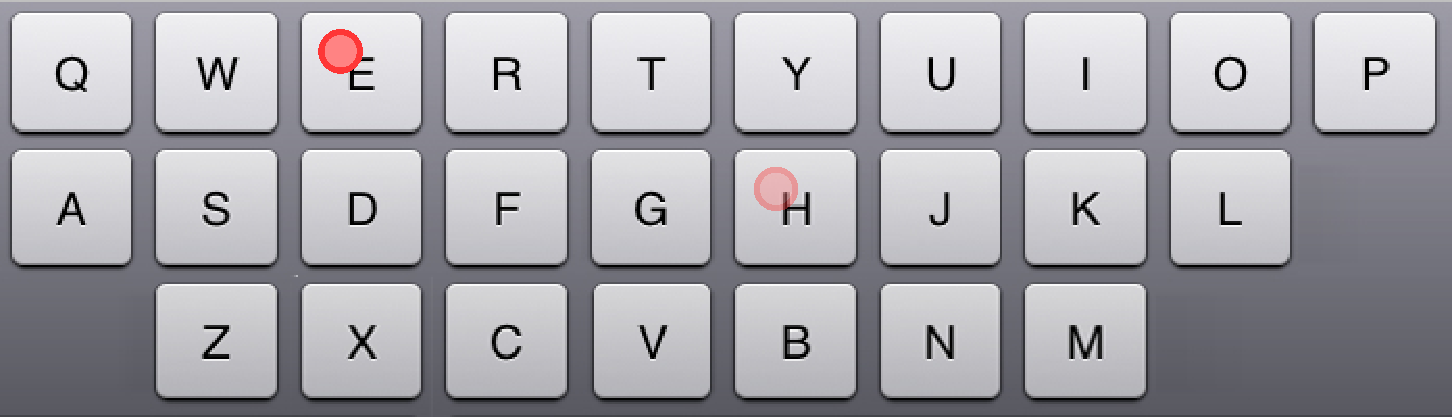
\includegraphics[width=1\columnwidth]{figures/26-Tap}

  \caption{The 26-Key tap keyboard design.}
  ~\label{fig:multiword}
\end{figure}

\subsection{Design \#4 - 26-Key Tap}

In this experiment, we explore how feedback can be added to a soft keyboard on the mobile phone to make it usable in virtual reality.
We want to explore the limit of touch typing and muscle memory for a user in a virtual enviroment.
We build a prototype keyboard, shown in Figure~\ref{fig:gesture}, for a mobile phone that transmits to the head-mounted display when where the user touches on the keyboard.
In this way, the user gets feedback where a finger is located on the keyboard with every tap.
The prototype keyboard is running alongside the standard Android keyboard that includes autocorrect to adjusted for typos and phonetic misspelling.

We notice an unexpected phenomenon using this prototype.
Even hitting the same key twice is difficult.
Every time a user lifts a finger and lowers the finger, there is a nontrivial chance that the finger has drifted to another key.
Even though the keyboard layout is familiar, and even error correction is applied, the error rate in this method make it unusable.
From this experiment, we hypothesize that for fine motor skills, some degree of either visual or haptic feedback is needed.


\begin{figure}[!htb]
  \centering

  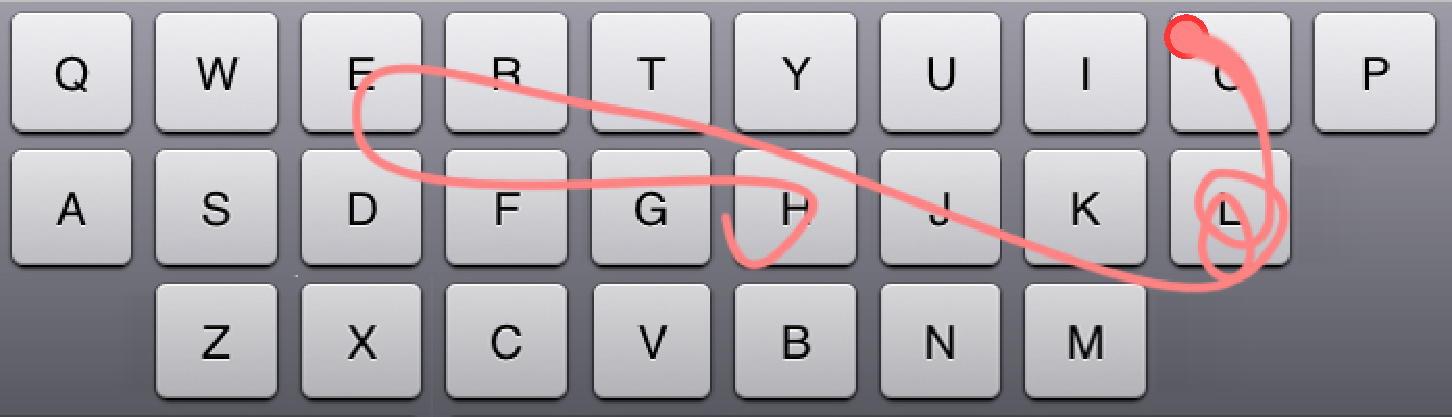
\includegraphics[width=1\columnwidth]{figures/gesture}
  
  \caption{The 26-Key gesture keyboard design.}
  ~\label{fig:gesture}
\end{figure}

\subsection{Design \#5 - 26-Key Gesture}


Gesture keyboards are shown to be effective in speeding up typing on mobile devices.
Since it does not involve lifting the finger, we postulated that it may also be useful in virtual reality.
Similar to the 26-key tap, the layout of the mobile QWERTY keyboard is preserved, except tapping is replaced by dragging to specific keys.
We show the virtual keyboard and gesture trail to indicate where the finger was in the virtual enviroment, shown in Figure~\ref{fig:gesture}.
We find that gestures works better than tapping.  However, there are two main problems: 

Firstly, the users cannot get the first letter right when starting the gesture.  We modify the shape recognition algorithm to as follows.  When the user puts their finger on the mobile screen, it always starts in the center.
The first inflection point is then discarded and the rest of the input is then done at the mobile phone system level using the standard gesture keyboard.

However, the speed with which the user creates gestures with the head-mounted display on is around three times slower than with the head-mounted display off.
Even for users that are familiar with gesture keyboards on their mobile phone, it is difficult for them to generate gestures in an efficient manner in virtual reality.
%Shape, location, and bi-gram modeling is used by SHARK2~\cite{kristensson2004shark} to generate the n-best outputs.

In summary, the use of gesture keyboard over a conventional keyboard is the best among the choices we explored in the initial phase.
Nonetheless, the speed of around 23 words per minutes, with the help of auto-correction, is still lower than desired.


\begin{comment}
>
\subsection{Design \#4 - 8-key Drag}
\vspace*{.1cm}
\includegraphics[width=.9\columnwidth]{figures/26Tap}

QWERTY keyboard is broken into 8 regions instead of 6.
User interact with this keyboard through dragging.
Both hands are required, with each hand dragging four directions (left, up, right, down) to input the 8 regions.

\subsection{Design \#5 - 6-key Tap}
\vspace*{.1cm}
\includegraphics[width=.9\columnwidth]{figures/26Tap}

This is our first design utilizing batched keys. QWERTY keyboard is divided into 6 sections. Tapping corresponding regions triggers input for a whole section.
A word recommender algorithm in back end is required.


\subsection{Design \#6 - 6-key Drag}
\vspace*{.1cm}
\includegraphics[width=.9\columnwidth]{figures/26Tap}

Similar to 6 keys tap, the method of interaction is changed to drag instead of tap.
A word recommender algorithm in back end is required.

Even though there can be realistic representation of the keyboard and his fingers in VR, users still suffer from not being able to see some part of his own body.
The solution to such visual segmentation is not apparent, for whole body tracking in VR is not yet available.

Studies show that users possesses approximate knowledge of where their fingers are on screen thanks to proprioception \cite{boff1986handbook}.

\section{Design Goals}
Before describing the prototypes and lessons learned, we present five high-level design goals that focus on input metrics, user experience, and adaptability.
These goals are informed by related work and our experience building other systems.

\subsection{Efficient}
How closely does the new device approach exceed the speed of the best devices for text input in virtual reality?

\subsection{Learnable}
How long does the device take to learn?
Does it rely on existing skills?
Is there ways for the user to transition from being a novice to an expert?

\subsection{Practical}
Is the input method usable today?
Moreover, will it be usable in the future given the where we think virtual reality controller are heading?

\subsection{General}
Is the text input method useful across multiple types of applications?
Can the user type their username, password, and a message to a friend?

\subsection{Usable}
Desktop user sessions are longer than mobile~\cite{Kamvar:2009:CIM:1526709.1526817}.
We hypothesize that virtual reality will have a user session time closer to that of a desktop computer than a mobile phone.
Once a user has take the time to wear the head mounted display and controller, the session will
Will the user be able to use the text input method comfortably?
Can they use it for as long as they use as they their computer at night?


\end{comment}


\section{Design Concepts}

We learned from our investigation that it is slow for users to hit the right key on a virtual keyboard due to the lag in visual feedback and limited proprioception.   We thus propose Slide, described below, to speed up text entry by using relative positioning and reducing the need for accuracy through auto-correction. 

\begin{comment}

Our design efforts focused on balancing three of the above factors: input speed, learning time, and physical size.
Our thinking was particularly influenced by the interaction design of cell phones that use T9 input, which relies on a database of words to disambiguate cell phone keypad keystrokes that are associated with more than one letter.
If we could design an input device that combined the best of the standard keyboard (fast text input, familiar layout) and the 12-key cell phone keypad (small size), we would have a device that could be used in off-the-desktop situations, potentially for extended typing tasks, with little degradation in performance. 

Despite the difficulties for the users to physically locate their finger outside of the virtual environment in order to interact with the keyboard on a mobile phone, the users are not completely helpless from their previous typing experience.
To start with, the users have muscle memory from typing on traditional mobile keyboards. With this previous experience, the user remembers, although imprecise, the location of letters if the layout of the keyboard is the same as what they are used to.

Thus, to leverage these previous knowledge of the users and address the problem that the users cannot physically see their fingers, we center our designs around two key features that we believe can help them adjust to typing in virtual reality: relative finger tracking, and batched keys.

Traditional mobile keyboard requires users to tap on the key precisely to enter an individual letter.
This method falls prey to specifically to the problem described above: users cannot tap on the individual keys accurate enough because they cannot see their finger relative to the touch screen of the mobile phone in a virtual environment.
Thus, 
\end{comment}

\subsection{Relative Vectors as Key Entries}

To minimize the need for visual feedback, we propose to use relative positioning.  Relative movement, instead of absolute, has also been found to be beneficial in reducing fatigue~\cite{Hincapie-Ramos:2014:CEM:2556288.2557130} so the user can start the interaction from their current position. 

The virtual keyboard in Slide is laid out exactly as the original keyboard, so the users are already familiar with the placement of the keys.   The positioning of the keyboard is relative to the user’s first touch.  No matter where the finger is placed on the touchpad, it is assumed to touch the center of the keyboard, right between the F and G letters.  To enter a letter, the user slides his finger to the key of interest.  As he lifts his finger, the key is entered.  Because of the familiarity of the keyboard layout, the user knows roughly even without looking at the keyboard.  Visual feedback is provided by showing the virtual keyboard and the trail his finger makes.   

Text entry in Slide is different from swiping in several important ways. 
\begin{enumerate}
\item
With swiping, the user enters a word through a continuous movement, connecting pairs of consecutive letters.  Without good visual feedback, the drift in our sense of our finger position accumulates with each letter.   With Slide, every letter input is independent.  The user needs only to slide always from the center of the keyboard to the letter of interest.  

\item 
As discussed above, we need to discard the first letter entry when we swipe in VR, since users cannot hit the first key correctly.   No such special provision is needed for Slide.

\item
With swiping, the worst-case distance traveled for each letter is the full length of the keyboard.  The worst case in Slide is just half the length of the keyboard. 
\end{enumerate}


\subsection{Directions as Key Entries}

\begin{figure}
  \centering

  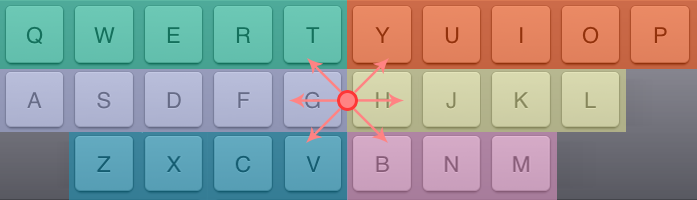
\includegraphics[width=1\columnwidth]{figures/arrows}
  
  \caption{The six tiles of the direction-based keyboard.}
  ~\label{fig:swipeVRLayout}
\end{figure}

While an improvement over swiping, the technique proposed above still requires the user to slide his finger precisely to the right key, which can be half the length of the keyboard.  We reduce the accuracy required of the user by relying on auto-correction.  We divide the keyboard into 6 tiles, as shown in Figure~\ref{fig:swipeVRLayout}.   The user only needs to slide his finger in the direction of the tile that contains the key of interest.  It is easy to indicate the direction accurately, with a minimum distance traveled for all keys, without visual feedback. 

We use a Bayesian word recommender to infer the most probable words among words that correspond to the same tile sequence.  For example, the words ``hello'' and ``jelly'' has the same representation.  
This recommender algorithm use 2-gram and 3-gram data from Google Books Ngram Viewer\footnote{http://storage.googleapis.com/books/ngrams/books/datasetsv2.html}, part of speech frequency for English dictionary, individual word frequency for the entire English language, and produces a prediction score.
The word with highest prediction score will be selected by default as the most probable word.  
The whole word is presented all at once, instead of a letter at a time, and the user is given the option to choose a less probable word among the possibilities, as shown in Figure~\ref{fig:multiword}.  


\begin{figure}
  \centering

  \includegraphics[width=.4\columnwidth]{figures/multiword}
  
  \caption{Users are presented with words represented by the same sequence of tile inputs.}
  ~\label{fig:multiword}
\end{figure}

\subsection{A Hybrid Keyboard}

While the directional approach is faster, it lacks the precision necessary for entering numbers, punctuations, or words not in the dictionary, such as user names, passwords, and URLs.   Our solution is to use the relative-vector technique as a backup for the direction-based keyboard.  Since both these techniques have the same keyboard layout, the user simply can mix these two entry techniques easily.  Our keyboard automatically detects the user’s intention based on the speed with which the keys are entered. 

In addition, we introduce a few shortcuts for the frequently used “delete” and “space” keys.   Users can double tap the touch screen to indicate delete.  For the space key, the user can click a specific physical button on the controller, such as the “trigger” button on the bottom side of the Vive controller.  We have also experimented automatically inserting a space after a certain timeout period between 150 and 500 ms.  However, we found that users preferred to have the control of when to insert the space themselves.   

\begin{figure*}
  \centering
  \includegraphics[width=1.75\columnwidth]{figures/map}
  \caption{Example of the system.  When the user want to type .}
  ~\label{fig:example}
\end{figure*}



\begin{comment}

\begin{figure}
\centering

  \begin{tikzpicture}

  \def \n {5}
  \def \radius {3cm}
  \def \margin {8} % margin in angles, depends on the radius

  \foreach \s in {1,...,\n}
  {
    \node[draw, circle] at ({360/\n * (\s - 1)}:\radius) {$\s$};
    \draw[->, >=latex] ({360/\n * (\s - 1)+\margin}:\radius) 
      arc ({360/\n * (\s - 1)+\margin}:{360/\n * (\s)-\margin}:\radius);
    }
  \end{tikzpicture}

  \caption{
    Controller\\
  Intent Detection Classifier\\
    triager \\
  |swipe          |                |\\
    ngram           deterministic     \\
    selection        letter           \\
}~\label{fig:systemFlowchart}
\end{figure}
\end{comment}


\subsection{Variations of Slide}
 
To arrive at the proposed design above, we have tried a few other variations, summarized below. 

\begin{enumerate}
\item
6-tile design and tapping with absolute positioning.  As in Slide, we divide the keys into 6 tiles, and users are asked to just tap on the corresponding tile.  We found that users still cannot hit the right tile, if we adopt absolute positioning.

\item
6-tile design and swiping with absolute positioning.  This design is faster that swiping on a 26-key keyboard, but it is still slower than our proposal. 

\item 
8-tile design with two cursors, and relatively positioning.  Since most people type with two hands on the keyboard, we experimented introducing two cursors into the proposed design.  We split the keyboard into the left and right half, and the initial positions of the left and right thumbs are assumed to be the center of each half.  Instead of sliding to one of 6 directions for each hand, we simplify it to four directions each (up, down, left,  right).  By having 8 rather 6 tiles, this can also reduce the number of ambiguous entries and improve the success of error correction.  

Testing it on a few users quickly pointed out the flaw of this design.  It is too complicated, as the user has to decide which thumb to use, and then which of the four directions.  Furthermore, we found that with the original proposal, the user typically uses the other hand to enter the special the special keys.
\end{enumerate}

Because none of the variations come close to the proposed entry method, our evaluation below focuses primarily on understanding the characteristics of our proposal. 


%\input{swipevr.tex}
\section{Evaluation of Slide}

\subsection{Participants}
Fifteen subjects, 5 female and 15 male, participated in the study.
All were university students and active users of technology.  
Each subject took about 30 minutes to complete the study.

\subsection{Measures}
In the field of text entry, several metrics are used to characterize a method's performance ~\cite{wobbrock2007measures,arif2009analysis}.
Here, we discuss the performance metrics we use to evaluate the performance of the input device.  

\subsubsection{Words per Minute}
Words per minute ($WPM$) is perhaps the most widely reported empirical measure of
text entry performance~\cite{wobbrock2007measures}:

\[ 
WPM={\vert T\vert -1\over S}\times 60\times{1\over 5}. \eqno{\hbox{(1)}}
\]

Where, $S$ is the time in seconds from the first key press to the last, which means that the entry of the first character is never timed, which is the motivation for the ``- 1'' in the numerator of Equation $1$ ~\cite{yamada1980historical}.
English words by convention are treated as having five characters~\cite{yamada1980historical}.

\subsubsection{Error Rate}
Error Rate ($ER$) is the ratio of the total number of incorrect characters in the transcribed text to the length of the transcribed text:

\[
ER={INF\over \vert T\vert }\times 100\%. \eqno{\hbox{(2)}}
\]

Where, Incorrect Not Fixed ($INF$) is the number of unnoticed incorrect characters in the transcribed text.

\subsection{Experiment \#1 - 26-Key Slide Keyboard}

Our first experiment is to measure the speed at which users can type in uncommon English words.  The user has to slide his finger to the specific keys to enter the characters precisely.  There is no auto-correct used in this mode as the primary use is for words that are not in the language model.  

In this experiment, the users were asked to type in two phrases: one that contained a proper noun and one that contained an abbreviation.  We found that the users can enter these phrases with an average entry rate of 12 WPM, with a standard deviation of 1.8.  We observed that practice has no significant effect on improving the speed. 
12 words per minute is a reasonable input rate, considering that input words are uncommon, and errors in entry cannot be corrected automatically. 


\subsection{Experiment \#2 - 6-tile Slide Keyboard}

For this experiment, we selected fifty phrases from a collection of five-hundred phrases commonly used for text entry evaluations~\cite{mackenzie2003phrase}.
Example of phrases from the set are ``video camera with a zoom lens'', ''have a good weekend'', and''what a monkey sees a monkey will do''.
To allow for cross-comparison to other text entry methods, the corpus doesn't include phrases with punctuation marks.
Non-alphanumeric symbols are rarely considered in text input research~\cite{mackenzie2003phrase} even though some punctuations (. - ' ( ) ") are more frequent than the least common English letter,  \textit{q}~\cite{malikpunctuation}.
 
Copying pre-selected phrase is usually the preferred method for text entry when doing evaluations in a lab setting~\cite{mackenzie2002character, mackenzie2003phrase}.
Although, copying pre-selected entry rates should be regarded differently from true, ``in the wild'' results when the user is composing text instead of transcribing prompted phrases.


One of our metrics in the experiment is the learnability of the system so we don't give users practice trials before beginning the actual test.
For each user we conduct twelve sequential sessions.
In each session, a user enters six phrases.
%After entering all the phrases with both input methods, the participant filled out
%a questionnaire regarding their quantitative feedback on the text entry method.
%Finally, subjects were asked for additional comments.


\begin{comment}

\begin{figure}
\centering

\begin{subfigure}{1\columnwidth}
  \begin{tabular}{@{}p{7cm}p{1cm}@{}}\toprule
  \textbf{Performance}                      &         \\
  \midrule
   The input device is responsive           &     $3.4$   \\
   The input device worked properly           &     $4.3$   \\
   The visuals are  smooth and don't freeze       &     $3.7$   \\
  \bottomrule
  \end{tabular}
  \caption{Overcoming latency is a main challenge for high bandwidth tasks in virtual reality. 
  Users find the input device works properly and is responsive.}
  \label{fig:performance}
\end{subfigure}


\vspace{4mm} 

\begin{subfigure}{1\columnwidth}
  \begin{tabular}{@{}p{7cm}p{1cm}@{}}\toprule
  \textbf{Design}                                 &     \\
  \midrule
  I understand how input device works                   &   $3.1$ \\
  It is easy to learn how to use the input device             &   $3.9$ \\
  I understand the graphical interface                    &   $3.9$ \\
  The text and input are clearly visible                  &   $2.7$ \\
  \bottomrule
  \end{tabular}
  \caption{Users agree that they understood how the input device and the graphical interface worked.
  Some found the text to be not clearly visible.}
  \label{fig:design}
\end{subfigure}


\vspace{4mm} 


\begin{subfigure}{1\columnwidth}
  \begin{tabular}{@{}p{7cm}p{1cm}@{}}\toprule
  \textbf{Applicability}                  &           \\
  \midrule
  I would use the input device to do a web search &     $3.3$     \\
  I would use the input device to write a note    &     $2.9$     \\
  I would use the input device at home        &     $3.2$     \\
  \bottomrule
  \end{tabular}
  \caption{User agreed that the Slide input device could be used to do a web search, write a note, and used at home. }
  \label{fig:controllerVive}
\end{subfigure}

  \caption{We ask the user to evaluate the performance, design, ergonomics and applicability of Slide on a 5-point Likert Scale (Strongly Disagree, Disagree, neutral, Agree, Strongly Agree).}
  
  \label{table:usability}

\end{figure}


\subsubsection{Subjective }
we ask the user to evaluate each entry mechanism on a 5-point Likert Scale (Strongly Disagree, Disagree, neutral, Agree, Strongly Agree).
Additionally, users are  interviewed to further understand the their qualitative experience.
\end{comment}

The collective learning curve is shown in Figure~\ref{fig:learnability}.
The mean starting rate for all users was 18 WPM.
Every user improved their WPM rate by at least 20\% from their starting rate.
To calculate the steady state average rate for text entry, we discard the first six sessions and find the steady state rate is 34 WPM with a standard deviation of 6.3. The average error rate for text entry was 4\% with a standard deviation of .018.




\begin{figure}
\centering

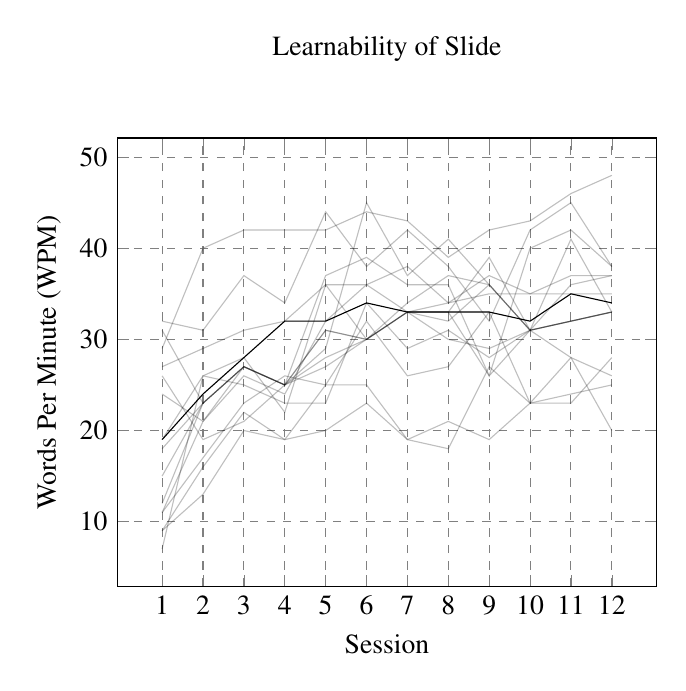
\begin{tikzpicture}
\pgfplotsset{
    every axis legend/.append style={
      at={(0.5,1.03)
    },
    anchor=south
    }
}
\pgfplotsset{grid style={dashed,gray}}

\begin{axis}[
legend columns=-1,
xlabel=Session,
ylabel=Words Per Minute (WPM),
 title style={at={(0.5,0)},anchor=south,yshift=180},
 title = Learnability of Slide,
 %ytick={0,5,10,15,20},
 %minor ytick={1,2,3,4,5,6,7,8,9,10,11,12,13,14,15,16,17,18,19,20},
 xtick={1,2,3,4,5,6,7,8,9,10,11,12},
 %minor xtick={1,2,3,4,5,6,7,8,9,10,11,12,13,14,15,16,17,18,19,20},
 grid=both,
]

\addplot[opacity=1] coordinates
{(1,19)(2,24)(3,28)(4,32)(5,32)(6,34)(7,33)(8,33)(9,33)(10,32)(11,35)(12,34)};
\addplot[opacity=0.25] coordinates
{(1,12)(2,23)(3,27)(4,25)(5,31)(6,30)(7,33)(8,33)(9,39)(10,31)(11,32)(12,33)};
\addplot[opacity=0.25] coordinates
{(1,24)(2,21)(3,26)(4,24)(5,32)(6,36)(7,33)(8,34)(9,35)(10,35)(11,37)(12,37)};
\addplot[opacity=0.25] coordinates
{(1,31)(2,23)(3,27)(4,25)(5,29)(6,45)(7,37)(8,41)(9,36)(10,31)(11,41)(12,33)};
\addplot[opacity=0.25] coordinates
{(1,29)(2,40)(3,42)(4,42)(5,42)(6,44)(7,43)(8,39)(9,42)(10,43)(11,46)(12,48)};
\addplot[opacity=0.25] coordinates
{(1,9)(2,16)(3,22)(4,19)(5,25)(6,32)(7,26)(8,27)(9,33)(10,23)(11,23)(12,28)};
\addplot[opacity=0.25] coordinates
{(1,27)(2,29)(3,31)(4,32)(5,36)(6,36)(7,38)(8,34)(9,37)(10,35)(11,35)(12,35)};
\addplot[opacity=0.25] coordinates
{(1,9)(2,13)(3,20)(4,19)(5,20)(6,23)(7,19)(8,18)(9,27)(10,23)(11,24)(12,25)};
\addplot[opacity=0.25] coordinates
{(1,11)(2,17)(3,23)(4,26)(5,25)(6,25)(7,19)(8,21)(9,19)(10,23)(11,28)(12,20)};
\addplot[opacity=0.25] coordinates
{(1,18)(2,23)(3,27)(4,25)(5,28)(6,30)(7,33)(8,32)(9,36)(10,31)(11,32)(12,33)};
\addplot[opacity=0.25] coordinates
{(1,26)(2,19)(3,21)(4,25)(5,37)(6,39)(7,36)(8,36)(9,26)(10,40)(11,42)(12,38)};
\addplot[opacity=0.25] coordinates
{(1,15)(2,23)(3,27)(4,25)(5,31)(6,30)(7,33)(8,33)(9,26)(10,31)(11,32)(12,33)};
\addplot[opacity=0.25] coordinates
{(1,19)(2,26)(3,28)(4,22)(5,36)(6,30)(7,34)(8,37)(9,36)(10,31)(11,36)(12,37)};
\addplot[opacity=0.25] coordinates
{(1,7)(2,26)(3,25)(4,23)(5,23)(6,34)(7,29)(8,31)(9,28)(10,31)(11,28)(12,26)};
\addplot[opacity=0.25] coordinates
{(1,11)(2,21)(3,27)(4,25)(5,27)(6,30)(7,33)(8,30)(9,29)(10,31)(11,32)(12,33)};
\addplot[opacity=0.25] coordinates
{(1,32)(2,31)(3,37)(4,34)(5,44)(6,38)(7,42)(8,38)(9,32)(10,42)(11,45)(12,38)};

\end{axis}
\end{tikzpicture}

%4.7.1 Markers for graph fixing the circle, square, x, triangle overloading

\caption{
Graph of learnability for the 6-tile Slide keyboard.
Entry rate on each block of 20 sentences.
Each line is a single participant.
}~\label{fig:learnability}
\end{figure}





\begin{comment}

\begin{figure}
\centering
  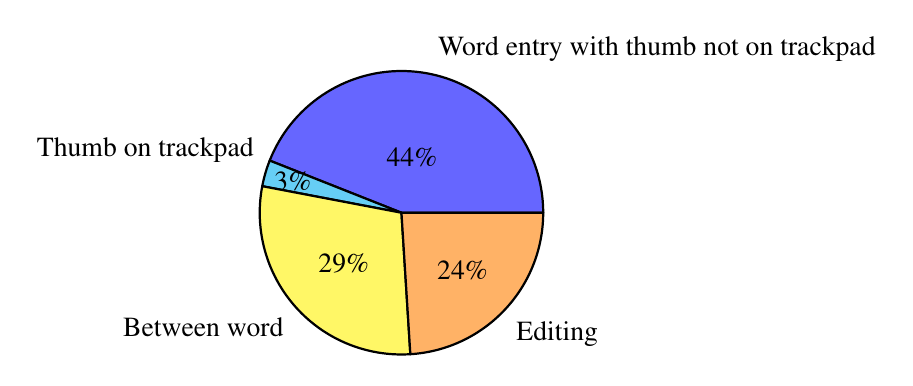
\begin{tikzpicture}[scale=.6]

      \pie{44/Word entry with thumb not on trackpad, 3/Thumb on trackpad, 29/Between word, 24/Editing}[explode=0.1]
  \end{tikzpicture}
  \caption{The majority of time the user was entering a word, their thumb was not on the trackpad.  There was also a delay between when the user was entering words.
    }
  ~\label{fig:distance}
  \end{figure}


\begin{figure}
\centering
\includegraphics[width=0.5\columnwidth]{figures/circle}
  \caption{Sample of a right-handed users' slides.  Slides are concentrated in the upper-left quadrant of the circular trackpad.}

\label{fig:circle}

\end{figure}

\begin{figure}
\centering
\begin{comment}


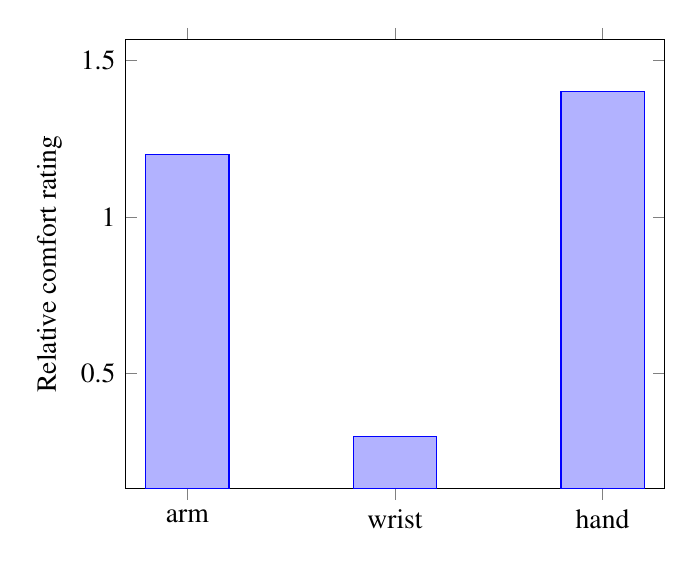
\begin{tikzpicture}
\begin{axis}[
    ybar,
    bar width=30pt,
    enlargelimits=0.15,
    ylabel={Relative comfort rating},
    symbolic x coords={arm,wrist,hand},
    xtick=data,
    ]
\addplot coordinates {(arm,1.2) (wrist,.3) (hand,1.4)};
\end{axis}
\end{tikzpicture}

  \caption{
 Differences between the initial and final subjective comfort ratings.  
    }
\label{fig:graphLearning}
\end{figure}
\end{comment}



%\input{future.tex}
\section{Conclusion}

\subsection{Overcomes Latency and Proprioception with Slide}


The lack of proprioception in virtual reality is compounded by the latency in visual feedback.
For a user to be able to steer their finger to a key, the time needed to transmit information from the real to virtual and back to the ``real'' through the  screen and into the eyes of the user is too long.  Other commonly used input methods, such as gesture keyboards, are subject to the same problem.
Therefore, we devise a method of input that does not depend on a feedback loop that requires the user to reach an absolute position on a keyboard.  

Our technique only depends on relative movement. The user slides the finger on the touchpad to indicate the relative position of the key of interest with respect to the center of the keyboard.  We further reduce the precision required by grouping keys into 6 tiles, and the user only needs to indicate the direction of the tile, again, with respect to the center of the keyboard.
This reframes the domain of text input from a closed  feedback control problem to an open feedback control problem.
As such we have created a system that lets users enter text in virtual reality efficiently.  With the help of error correction, and including the time of error correction, users can type at about 34 words per minute with an error rate of 4\%.  Furthermore, when precision is desired, the user can simply go slower and hit the precise keys.  The user can still precisely, which is useful for passwords, etc, at a rate of 12 words per minute. 

\subsection{Smooth Transition From Newbie to Novice to Expert }

A smooth pathway learnability is an important factor for an input device to gain widespread adoptability.
Some users will immediately reject an input device that requires too much up front practice before it becomes useful.
Slide has a natural path to transition novice (low threshold) to expert (high ceiling) users~\cite{grover2013computational}.

Slide offers a clear path from newbie to novice to expert. 
Slide is instantly usable: newbie users can use the system quickly by looking at the controller and slowly moving their thumb to a key.
Novice users would periodically glance down to look at the virtual keyboard if they forget the position of a key. 
With a little of practice, users can remember the location of the keys.  
Experts can just type without having to look at the virtual keyboard. 

\subsection{General-Purpose Text Entry}
As virtual reality matures, we expect VR systems to have a standard text-entry method at the OS level, that can be learned once and used across applications. 
This is analogous to the adoption of a pointing device for PCs.  This text-entry method must be general-purpose, accommodating the entry of 
proper nouns, abbreviations, capital letters, colloquialism, passwords, etc. 
Allowing both fast entry of common words and precise, albeit slower, of the characters, Slide is positioned well as a candidate for the keyboard of a VR operating system.        

\begin{comment}
\subsection{Accessibility}
Virtual reality gives access access to something that they might never see in real life.
But for a disabled person, virtual reality might be the path to inclusion.
SwipeVR can be adapted for assistive technology products such as wands, joysticks, trackballs, touch screens.


\subsection{End}

concluding notes
\\
We present a fast text entry input device for virtual reality.
It is faster than the state of the art.
It can be used in public.
It dosnt tire your arms or vocal chords.

Using virtual reality for programming is a rich area for further discovery.
The large workspace that virtual reality provides is received well by users.

They keyboard is currently the weak point in many virtual reality applications.

Touch-typing on the keyboard is difficult as is switching context between the virtual reality controllers and the keyboard.

In the future, high-quality virtual reality headsets will be standalone devices, not tethered to desktop computers \cite{schaller1997moore}.
As the price of headsets decrease \cite{brown2016virtual}, virtual reality is positioned to become a democratizing technology.
Thus it is a worthwhile endeavour to determine how to program in virtual reality, both as a teaching tool for novices and as a more expressive tool for experts.

\end{comment}




% Use a numbered list of references at the end of the article, ordered
% alphabetically by first author, and referenced by numbers in
% brackets~\cite{ethics, Klemmer:2002:WSC:503376.503378,
%   Mather:2000:MUT, Zellweger:2001:FAO:504216.504224}. For papers from
% conference proceedings, include the title of the paper and an
% abbreviated name of the conference (e.g., for Interact 2003
% proceedings, use \textit{Proc. Interact 2003}). Do not include the
% location of the conference or the exact date; do include the page
% numbers if available. See the examples of citations at the end of this
% document. Within this template file, use the \texttt{References} style
% for the text of your citation.

% Your references should be published materials accessible to the
% public.  Internal technical reports may be cited only if they are
% easily accessible (i.e., you provide the address for obtaining the
% report within your citation) and may be obtained by any reader for a
% nominal fee.  Proprietary information may not be cited. Private
% communications should be acknowledged in the main text, not referenced
% (e.g., ``[Robertson, personal communication]'').







% Balancing columns in a ref list is a bit of a pain because you
% either use a hack like flushend or balance, or manually insert
% a column break.  http://www.tex.ac.uk/cgi-bin/texfaq2html?label=balance
% multicols doesn't work because we're already in two-column mode,
% and flushend isn't awesome, so I choose balance.  See this
% for more info: http://cs.brown.edu/system/software/latex/doc/balance.pdf
%
% Note that in a perfect world balance wants to be in the first
% column of the last page.
%
% If balance doesn't work for you, you can remove that and
% hard-code a column break into the bbl file right before you
% submit:
%
% http://stackoverflow.com/questions/2149854/how-to-manually-equalize-columns-
% in-an-ieee-paper-if-using-bibtex
%
% Or, just remove \balance and give up on balancing the last page.
%
\balance{}


% REFERENCES FORMAT
% References must be the same font size as other body text.
\bibliographystyle{SIGCHI-Reference-Format}
\bibliography{sample}

\end{document}

%%% Local Variables:
%%% mode: latex
%%% TeX-master: t
%%% End:
